\documentclass[11pt]{article}

\title{\color{dark-maroon} Differences-in-Differences with Spatial Spillover}
% \subtitle{Subtitle}
\author{\normalsize Kyle Butts\\{\footnotesize Univ. of Colorado, Boulder}}
\date{\footnotesize\today}

% Margins ----------------------------------------------------------------------

\usepackage[margin=1.25in]{geometry}

% AMS --------------------------------------------------------------------------

\usepackage{amsmath}
\usepackage{amsfonts}
\usepackage{amsthm}
\usepackage{graphicx}


% Line Spacing -----------------------------------------------------------------

\renewcommand{\baselinestretch}{1.5}


% Font -------------------------------------------------------------------------

\usepackage[T1]{fontenc}
\usepackage[default]{lato} % Lato as text font
% \usepackage[utopia, varg]{newtxmath}
% \renewcommand{\rmdefault}{futs} % Utopia as text font 

% Small adjustments to text kerning
\usepackage{microtype}

% Remove annoying over-full box warnings
\vfuzz2pt 
\hfuzz2pt


% Tikz support -----------------------------------------------------------------

\usepackage{tikz}


% Color Palette ----------------------------------------------------------------

\usepackage{xcolor}

% https://www.materialpalette.com/colors
\definecolor{dark-maroon}{HTML}{5D0F0D}
\definecolor{navyblue}{HTML}{0A3044}

% From Davidson Mackinnon
\definecolor{dm-blue}{HTML}{086fbd}
\definecolor{dm-red}{HTML}{ba3132}
\definecolor{dm-green}{HTML}{3f7e32}

% https://www.viget.com/articles/color-contrast/
\definecolor{purple}{HTML}{5601A4}
\definecolor{navy}{HTML}{0D3D56}
\definecolor{ruby}{HTML}{9a2515}
\definecolor{alice}{HTML}{107895}
\definecolor{daisy}{HTML}{EBC944}
\definecolor{coral}{HTML}{F26D21}
\definecolor{kelly}{HTML}{829356}
\definecolor{cranberry}{HTML}{E64173}
\definecolor{jet}{HTML}{131516}
\definecolor{asher}{HTML}{555F61}
\definecolor{slate}{HTML}{314F4F}


% Hyperlinks -------------------------------------------------------------------

\usepackage{hyperref}
\hypersetup{
    colorlinks= true,
    citecolor= dark-maroon,
    linkcolor= dark-maroon,
    filecolor= dark-maroon,      
    urlcolor= dark-maroon,
}


% Citations --------------------------------------------------------------------

% note, natbib provides better hyperlinking
\usepackage{natbib}
\bibliographystyle{econ-aea}


% Define Theorems --------------------------------------------------------------

% Put proper spacing after Theorem #. 
\newtheoremstyle{spacing}
{}%          Space above, empty = `usual value'
{}%          Space below
{}%  Body font
{}%          Indent amount (empty = no indent, \parindent = para indent)
{\bfseries\color{navyblue}}% Thm head font
{.}%         Punctuation after thm head
{2.5mm}%  Space after thm head: \newline = linebreak
{}%          Thm head spec

% note, theorem is the name that goes in \begin{} and Theorem is the name displayed as Theorem 1
\theoremstyle{spacing}
\newtheorem{theorem}{Theorem}
\newtheorem{proposition}{Proposition}
\newtheorem{assumption}{Assumption}
\newtheorem{example}{Example}


% Custom Math Definitions ------------------------------------------------------

\newcommand{\expec}[1]{\mathbb{E}\left[#1\right]}%
\newcommand{\condexpec}[2]{\mathbb{E}\left[#1 \ \vert \ #2\right]}%
\newcommand{\prob}[1]{\mathbb{P}\left[#1\right]}%
\newcommand{\var}[1]{\mathrm{Var}\left[#1\right]}%
\newcommand{\cov}[1]{\mathrm{Cov}\left[#1\right]}%
\newcommand{\one}{\mathbf{1}}


% Titlepage --------------------------------------------------------------------

% \maketitle
\usepackage{titling}
\usepackage{setspace}

% title
\pretitle{\begin{spacing}{1}\begin{flushleft}\huge}
\posttitle{\end{flushleft}\end{spacing}\vspace{-5mm}}
% author, note don't use \and 
\preauthor{\begin{flushleft}\LARGE}
\postauthor{\end{flushleft}\vspace{-7.5mm}}
% date
\predate{\begin{flushleft}\Large\color{asher}}
\postdate{\end{flushleft}\vspace{-5mm}}

% Abstract
\renewenvironment{abstract}
 {\noindent\rule{\linewidth}{.5pt}\noindent}
 {\noindent\rule{\linewidth}{.5pt}}

% alternative abstract
% \renewenvironment{abstract}
% {
%   \centerline {\large \bfseries \scshape \color{navyblue} Abstract}
%   \begin{quote}
% }
% {\end{quote}}


% Section and Subsection Styling -----------------------------------------------

\usepackage[explicit]{titlesec}

\titleformat{\section}
  {\Large \bf \color{navyblue}}
  {\thesection \,---}
  {0.25em}
  {#1}
  
\titleformat{\subsection}
  {\fontsize{11}{10}\it}
  {\thesubsection.}
  {1em}
  {#1}

% Don't number subsubsection
\setcounter{secnumdepth}{2}

% Footnote ---------------------------------------------------------------------

% Spacing between footnotes on same page
\addtolength{\footnotesep}{1mm}

% Space after footnote number
\let\oldfootnote\footnote
\renewcommand\footnote[1]{\oldfootnote{\ #1}}

% No footnote line
\renewcommand\footnoterule{}

% No supsercript in footer
\makeatletter
\renewcommand\@makefntext[1]{%
    \parindent 1em \noindent
    \hb@xt@1.8em{\hss\normalfont\@thefnmark.\hfill}#1
  }
\makeatother




% Enumerate/Itemize ------------------------------------------------------------

\usepackage{enumitem}
\setitemize{labelindent=0.5em,labelsep=0.25cm,leftmargin=*}
\setenumerate{labelindent=0.5em,labelsep=0.25cm,leftmargin=*}


% Table and Figure labelling ---------------------------------------------------

\usepackage{caption}

\DeclareCaptionLabelSeparator{threedash}{\,---\,}
\DeclareCaptionFont{navyblue}{\color{navyblue}}
\DeclareCaptionFont{jet}{\color{jet}}
\captionsetup[table]{format=plain, labelsep=threedash, font={navyblue, bf}}
\captionsetup[figure]{format=plain, labelsep=threedash, font={navyblue, bf}}

% Alternative: Left align captions
% \captionsetup[table]{labelfont=it, textfont={navyblue, bf}, labelsep=newline, justification=raggedright, singlelinecheck=off}
% \captionsetup[figure]{labelfont=it, textfont={navyblue, bf}, labelsep=newline, justification=raggedright, singlelinecheck=off}

% multifigure with \caption
% \begin{subfigure}\caption{} \end{subfigure}
\usepackage{subcaption}
\captionsetup[subfigure]{format=plain, font={jet, footnotesize, bf}}


% Tables -----------------------------------------------------------------------

% Fix \input with tables
% \input fails when \\ is at end of external .tex file

\makeatletter
\let\input\@@input
\makeatother

% Make tables/figures wider than \textwidth using:
% \begin{adjustbox}{width = 1.2\textwidth, center}
% \end{adjustbox}
\usepackage{adjustbox}

% Slighty more spacing between rows
\usepackage{array}
\renewcommand\arraystretch{1.2}

% Table with easy to use footnotes
% \begin{threeparttable}
%    \begin{tabular} ... \end{tabular}
%    \begin{tablenotes}
%        \item \textit{Notes.}
%    \end{tablenotes}  
% \end{threeparttable}
\usepackage[flushleft]{threeparttable}
\setlength\labelsep{0pt}

% \toprule, \cmidrule, \bottomrule
\usepackage{booktabs}

% If tables are too narrow, fill columns using:
% \begin{tabularx}{\linewidth}{cols}
% col-types: X - center, L - left, R -right
% If you want relative scale for columns: 
% >{\hsize=.8\hsize}X/L/R
\usepackage{tabularx}
\newcolumntype{L}{>{\raggedright\arraybackslash}X}
\newcolumntype{R}{>{\raggedleft\arraybackslash}X}
\newcolumntype{C}{>{\centering\arraybackslash}X}

% Shorter multicolumn commands
\newcommand{\mcc}[1]{\multicolumn{1}{c@{}}{#1}}
\newcommand{\mcl}[1]{\multicolumn{1}{l@{}}{#1}}
\newcommand{\mcr}[1]{\multicolumn{1}{r@{}}{#1}}

% d column
\usepackage{dcolumn}
\newcolumntype{d}[1]{D..{#1}}

% Landscape table 
% \begin{landscape} \pagestyle{lscaped} table... \end{landscsape}
% \usepackage{pdflscape} - rotates page left-side up in pdf
% \usepackage{lscape} - does not rotate page, only figure/table

\usepackage{pdflscape}

% For landscape, fix page number location
\usepackage{fancyhdr}
\fancypagestyle{lscaped}{%
    \fancyhf{}
    \renewcommand{\headrulewidth}{0pt}
    \textnormal
    \fancyfoot{%
        \tikz[remember picture,overlay]
        \node[outer sep=2.5cm,above,rotate=90] at (current page.east) {\thepage};
    }
}
  

% ------------------------------------------------------------------------------

\usepackage[
    citestyle= authoryear,
    style= authoryear, 
    natbib= true, 
    backend= biber
]{biblatex}
\addbibresource{references.bib}

\usepackage{subcaption}

\begin{document}

% --------------------------------------------------
\begin{titlepage}
    \maketitle
    
    \begin{abstract}
        Empirical work often uses treatment variables defined by geographic boundaries. When researchers ignore the common problem that the effects of treatment cross over borders, differences-in-differences produces biased estimates for the average treatment effect. In this paper, I identify two sources of bias. First, the control group no longer identifies the counterfactual trend because their outcomes are affected by treatment. Second, changes in treated units' outcomes reflect the effect of their own treatment status and the effect from the treatment status of ``close'' units. I use Monte Carlo simulations to demonstrate when the biases are particularly large. Further, I show that a common solution used in the literature of removing `contaminated' control units only prevents one source of bias. Lastly, I propose improved estimation strategies that can remove both sources of bias.  
    \end{abstract}
\end{titlepage}
% --------------------------------------------------
    
\newpage 

% --------------------------------------------------
\section{Introduction}
% --------------------------------------------------

Empirical work in economics often considers treatment assigned by geographic boundaries such as cities, counties, and states. The effect of these treatments do not typically stay within these boundaries whether it be from people crossing borders or from general equilibrium mechanisms affecting neighboring areas. In the causal inference literature, the Stable Unit Treatment Value Assumption (SUTVA) is often assumed which says that treatment effects do not depend on the treatment status of any other unit \citep{Rubin_1980}. This article considers a common violation of SUTVA in a process I label `spatial spillovers' where `close' units treatment assignment affects outcomes of nearby units.\footnote{Close can refer to many different things, e.g. geographic distance, node distance in graph theory, or social relationships in schools or cities.} 

Despite the problem of spatial spillovers being common across many settings, \citet{Berg_Streitz_2019} document that little empirical analysis takes the problem seriously. In a survey of eight top Economics and Finance Journals in 2017, they find that only 21 articles out of 108 that run differencse-in-differences estimation discuss spillovers.\footnote{The articles surveyed are American Economic Review, Econometrica, the Journal of Political Economy, the Quarterly Journal of Economics, the Review of Economic Studies, the Journal of Finance, the Journal of Financial Economics, and the Review of Financial Studies.} Of those 21, only eight include spillovers to prevent bias in the estimation of treatment effects.

In the presence of these spatial spillovers, I identify two sources of bias that result when estimating treatment effects by standard differences-in-differences methodologies. First, untreated units that are `close' to treated units experience effects of treatment and therefore these `control' units fail to identify the counterfactual trend. When estimating by differences-in-differences, the spillover onto the `close' control units is averaged into the untreated change in outcomes. In this case, the spillover is subtracted from the estimated treatment effect and biases the estimate in the opposite sign of the spillover effect. For example, if a factory opening in a given county benefits both that county and neighboring counties, the treatment effect estimate is negatively biased because the change in outcome in neighboring counties is higher than it would be absent treatment. 

Second, changes in treated units' outcomes reflect the effect of their own treatment status and the effect from the treatment status of ``close'' units. Therefore the spillover is added to the treated units' change in outcomes. Therefore the bias of treatment effect is the same sign as the sign of the spillover. For example a factory opening in two neighboring counties might cause the benefit of each individual factory to decrease. The estimated treatment effect will be negatively biased because there is a negative spillover onto also treated units. 

The magnitude of the bias depends on two factors: the size of the spillover and the number of units affected by spillovers. If spillovers are quite large in magnitude or spread far over distance, then the bias will generally be large. This paper provides an explicit form for this bias and enables researchers to give bounds for it under assumptions about the size of the spillover effect and on number of units affected. I use Monte Carlo simulations to quantify the magnitude of bias in various spillover settings. 

\citet{Berg_Streitz_2019} find that six of the eight papers that include spillovers directly in their estimation strategy simply drop the control units they suspect to be affected by spillovers. Since this is a common strategy by researchers, I use Monte Carlo simulations to show that this method is effective in the case where there is \textit{only} spillovers on to control units. Dropping control unit observations, however, makes estimates less precise, so parameterizing the spillover function may be a better strategy especially in the case where there is a high proportion of control units neighboring treated units. 

@TODO: Paragraph on practical guidance on including spillover measures

% @TODO: Urban Application 

% --------------------------------------------------
\subsection{Literature Review}
% --------------------------------------------------

There are two different models of SUTVA violations in the literature. Within-group spillovers are when units are in distinct groups and outcomes depend on the treatment status of your group only. For example, SUTVA is violated if a person's likelihood of getting sick depends on the vaccine rate of his community. In this case, the community is the group within which spillovers can occur. Between-group spillovers occur when groups are overlapping which allows for more general forms of spillover. For example, a counties' economic outcomes depend on the economic outcomes of nearby counties (even across state borders). @TODO: Add citations for papers that find this.

One set of literature discusses `partial intereference' where spillovers are assumed to only occur within a group and not across groups.\footnote{\citet{Halloran_Struchiner_1995} considers community-vaccine rates in epidemology; \citet{Sobel_2006} considers interference in the Moving to Opportunity Program; and \citet{Angrist_2014} studies the context of school peer effects.} This setting compares ``control'' units in a partially treated group with control units in completely untreated groups to estimate spillover effects.\footnote{\citet{Angelucci_DiMaro_2016} provides a summary for estimation of within-group treatment effects.} However, the setting in my paper does not feature distinct groups which allow for the researcher to seperate areas into distinct non-overlapping groups.

\citet{Vazquez-Bare_2019} models within-group spillovers such that their exposure mapping is only a function of unit $i$'s group's treatment vector. He develops a potential outcomes framework which assumes that potential outcomes are a function of both own treatment-status $D_i$ and a function of the vector of treatment assignments $h_i(\vec{D})$ (this is referred to as an exposure mapping). Adding an exposure mapping to the potential outcomes framework allows to explicitly model SUTVA violations. Using this framework, he shows that a difference in means comparison between treated and control units is a biased estimated for the treatment effect. My paper uses this potential outcome framework in the case where treatment spillover is not limited to within-group spillovers and considers estimation of treatment effects by differences-in-differences. 

\citet{Sävje_Aronow_Hudgens_2019} consider a similar potential outcome framework as \citet{Vazquez-Bare_2019}, but they instead include spillovers as a part of their definition of ``treatment effect''. Then, the authors describe how the ATE estimated by diff-in-diff averages over both individual heterogeneity and, central to their contribution, over heterogeneity in the exposure mapping, $h_i(\vec{D})$. This paper develops a strategy to allow researchers to seperately identify treatment effects and spillovers.

The paper closest to mine is \citet{Delgado_Florax_2015} where they consider spillover only on to control units and identify a bias that can come from estimating a diff-in-diff model without explicitly controlling for spillovers. Using Monte-Carlo simulations, they find that there is an omitted variable bias problem by not including a measure of spillovers. This paper derives an explicit form for this bias in terms of potential outcomes and also includes the presence of spillovers on to also treated units.

Similarly, \citet{Clarke_2017} finds an explicit form for bias when estimating a diff-in-diff model with spillover onto control units. However, their model only allows spillovers onto control units and assumes spillovers are constant regardless on the number of nearby treated units. Lastly, \citet{Berg_Streitz_2019} and \citet{Verbitsky-Savitz_Raudenbush_2012} find results for a specific potential outcome function where $h_i(\vec{D})$ is the proportion of treated contiguous counties. They allow this spillover to enter the potential outcome additively and the coefficient is allowed to differ by own treatment status.

In my framework, if I assume the particular functional forms for potential outcomes of \citet{Clarke_2017}, \citet{Berg_Streitz_2019}, and \citet{Verbitsky-Savitz_Raudenbush_2012}, I arrive at the same bias equation as theirs. 

%%%%
The paper is structured as follows. ...









% --------------------------------------------------
\section{Potential Outcomes Framework}
% --------------------------------------------------

Assume there is a time $t_0$ where treatment turns on for all treated units and remains on afterwards. As in \citet{Vazquez-Bare_2019}, potential outcomes for unit $i$ at time $t$ are a function of own treatment-status $D_i$ and of a function of the vector of treatment assignments $h_i(\vec{D})$ where $\vec{D} \in \{0,1 \}^n$. This function $h_i(\vec{D})$ is referred to as an `exposure mapping' and is a non-negative scalar.\footnote{The derivation of bias does not require this assumption.} The function $h_i(\vec{D})$ measures the exposure to spatial spillover and no exposure to spatial spillovers is when $h_i(\vec{D}) = 0$.

To help better understand an exposure mapping, I give three examples of $h_i(\vec{D})$. Let $d(i,j)$ be a geographic distance measure which tells the distance unit $i$ is from unit $j$. First, $h_i(\vec{D})$ can be a 0/1 variable that equals one only if there is a treated unit within $x$-miles of unit $i$ (also commonly used is counties that share borders). In this case \[
    h_i(\vec{D}) = \max_{i \neq j} D_j * 1[ d(i,j) < x ] 
\] 
Second, $h_i(\vec{D})$ can be a function that equals the proportion of the k-nearest neighbors that are treated, i.e. \[
    h_i(\vec{D}) = 1/k \sum_{j \in k(i)} D_j,
\]
where $k(i)$ is the index of unit $i$'s k-nearest neighbors. Last, is the spatial decay function which depends on  the decay parameter $\alpha$. In this case, spillover intensity is the sum across all treated observations' decay term, i.e. \[ 
    h_i(\vec{D}) = \sum_{j \neq i} D_j \exp^{-\alpha d_i(j)}
\] 
The exposure mapping is part of the parameterization of spillovers, but the functional form of the potential outcome still needs to be specified. 



% --------------------------------------------------
\subsection{Spatial Spillovers}
% --------------------------------------------------

With a new definition of potential outcomes, I now formalize what is meant by ``spatial spillovers'. I define `spillover onto control units' as: \[
    Y_{i}(0, h_i(\vec{D})) - Y_{i}(0, 0).
\] 
Then, the average spillover onto control units averages over potential heterogeneity in spillovers and over heterogeneity in exposure intensity $h_i(\vec{D})$: \[
    \tau_{\text{spill,control}} = \mathbb{E}_i \left[ Y_{i}(0, h_i(\vec{D})) - Y_{i}(0, 0) \ \vert \ D_i = 0 \right].
\]
To emphasize, the average spillover effect depends on the average of exposure mapping. For example, assuming the potential outcomes is additively linear in $D_i$ and $h_i(\vec{D})$, then an individual control unit's spillover effect is $\beta_{\text{spill,control}} \ h_i(\vec{D})$. The average spillover onto control unit would therefore be $\tau_{\text{spill,control}} = \beta_{\text{spill,control}} * \mathbb{E}_{i} \left[ h_i(\vec{D})\right]$, i.e. the average over all control units exposure mapping.

Similarly, we define the spillover onto also treated units as: \[ 
    \tau_{\text{spill,treated}} = \mathbb{E}_i \left[ Y_{i}(1, h_i(\vec{D})) - Y_{i}(1, 0) \ \vert \ D_i = 1 \right].
\] 

It is important to clarify what I am assuming is the estimand of interest researchers would like to estimate when using differences-in-differences. I assume that the term `Average Treatment Effect' is trying to measure what I will call the `direct effect of treatment': \[
    \tau_{\text{direct}} = \mathbb{E}_i \left[ Y_{i}(1, 0) - Y_{i}(0, 0) \ \vert \ D_i = 1 \right],
\] 
which measures the effect of being treated in the absence of exposure to spillovers. This differs from \citet{Sävje_Aronow_Hudgens_2019} where they define the Average Treatment Effect as \[ 
    \mathbb{E}_i \left[ Y_{i}(1, h_i(\vec{D})) - Y_{i}(0, h_i(\vec{D})) \ \vert \ D_i = 1 \right],
\] 
where the expectation is over individuals and their exposures. I prefer the former because it allows for seperate identification of the direct effect of treatment and the spillover effects themselves.\footnote{The spillover effects themselves might be of interest to the researcher, so clearly seperating them is beneficial in estimation. Later they can be combined to estimate the `net effects' that \citet{Sävje_Aronow_Hudgens_2019} estimate.}


% --------------------------------------------------
\subsection{Bias in Differences-in-Difference Estimation}
% --------------------------------------------------

In this section, I identify the two sources of bias in differences-in-differences estimation. For exposition, I will refer to two periods, $t = 0$ and $t = 1$, but this can be replaced by averages across $Y$ in the pre-period and the post-period respectively. First, I present the equivalent to the parallel counterfactual trends assumption in the context of the new potential outcome framework. 

\begin{assumption}[Parallel Counterfactual Trends]\label{parallel}
    \[ 
        \mathbb{E}\left[ Y_{i1}(0, 0) - Y_{i0}(0, 0) \ \vert \ D_i = 1 \right] = 
        \mathbb{E}\left[ Y_{i1}(0, 0) - Y_{i0}(0, 0) \ \vert \ D_i = 0 \right]
    \]
\end{assumption}

This assumption states that in the absence of treatment and with zero exposure (not just the absence of individual $i$'s treatment), the change in potential outcomes from period 0 to 1 would not depend on treatment status. This generalizes to the typical Parallel Counterfactual Trends because typically SUTVA assumes that every unit has zero exposure.

When researchers run the canonical differences-in-differences regression \[ 
    y_{it}  = \alpha + \tau D_{it} + \epsilon_{it},
\]
$\hat{\tau}$ will be a biased estimate for $\tau_{\text{direct}}$.
Given that Assumption \ref{parallel} holds, the estimate can be decomposed as the direct effect and the two sources of spillover bias.

\begin{theorem}
    \label{thm:bias}
    If Assumption \ref{parallel} holds, 
    \begin{align*}
        \mathbb{E}[\hat{\tau}] &= \mathbb{E}\left[ Y_{i1} - Y_{i0} \ \vert \ D_i = 1 \right] - \mathbb{E}\left[ Y_{i1} - Y_{i0} \ \vert \ D_i = 0 \right] \\ 
        &= \tau_{\text{direct}} + \tau_{\text{spill,treated}} - \tau_{\text{spill,control}}
    \end{align*}
\end{theorem}

The intuition behind the biases are as follows. First, the change in outcomes among treated units combines the direct effect and the spillover from nearby treated units. Therefore the first difference adds the average spillover onto the treated units. Second, the change in outcomes among control units combines the parallel counterfactual trend with the average spillover onto control units. Since $\hat{\tau}$ is found by subtracting this second difference, we subtract the average spillover onto the control. 


% --------------------------------------------------
\subsection{Example Parameterization of Bias}
% --------------------------------------------------

To exemplify the above bias, I will model a particular form of spillovers by parameterizing the exposure mapping and the potential outcomes equation. For the exposure mapping, I will assume that spillovers occur for any county that is within 40 miles of a treated county, i.e. 
\begin{align}
    \label{eq:example_exposure}
    \text{Near}_{it} \equiv h_i(\vec{D}) = \max_{i \neq j} D_j * 1[ d(i,j) < 40 ].
\end{align}
This specification is a simple one in that the spillover is not additive in the number of nearby treated units and does not decay over distance. The potential outcome is assumed to be additive in both treatment and in the exposure mapping, but the coefficient on $\text{Near}_{it}$ is allowed to differ between treated and non-treated unitts:
\begin{align}
    \label{eq:example_po}
    \begin{split}
        y_{it} &= \alpha + \mu_t + \mu_i + \beta_{\text{direct}} D_{it} + \beta_{\text{spill,control}} (1-D_{it}) \text{Near}_{it} \\
        &\quad + \beta_{\text{spill,treated}} D_{it} \text{Near}_{it} + \varepsilon_{it},
    \end{split}
\end{align}
where $\mu_t$ and $\mu_i$ are unit and time fixed effects respectively. In this case, the spillover on an individual control unit is given by $\tau_{\text{spill,control}}$ and on an treated unit is $\tau_{\text{spill,treated}}$. 

If a researcher estimates 
\begin{align}
    \label{eq:twfe}    
    y_{it} = \alpha + \mu_t + \mu_i + \tau D_{it} + \varepsilon_{it},    
\end{align}
then the bias will be $\tau_{\text{spill,treated}} - \tau_{\text{spill,control}}$ where the two bias terms are \[ 
    \tau_{\text{spill,control}} = \beta_{\text{spill,control}} \frac{\sum_{i: D_{it} = 0} \text{Near}_{it}}{N_C}
\] and \[ 
    \tau_{\text{spill,treated}} = \beta_{\text{spill,treated}} \frac{\sum_{i: D_{it} = 1} \text{Near}_{it}}{N_T},
\]
where $N_C$ and $N_T$ are the number of control and treated units respectively. Simply put, the bias will be the proportion of treated units that receive spillover effects time the size of the effect on treated units minus the proportion of control units that receive spillover effects time the size of the effect on control units. 



% --------------------------------------------------
\section{Monte Carlo Simulations}
% --------------------------------------------------

% --------------------------------------------------
\subsection{Simulation 1}
% --------------------------------------------------

\begin{figure}[t]
    \caption{Bias of $\hat{\tau}$ with and without Control Units with Spillovers}
    \label{fig:bias_as_treat_prob}
    {\centering
        \resizebox{\columnwidth}{!}{
            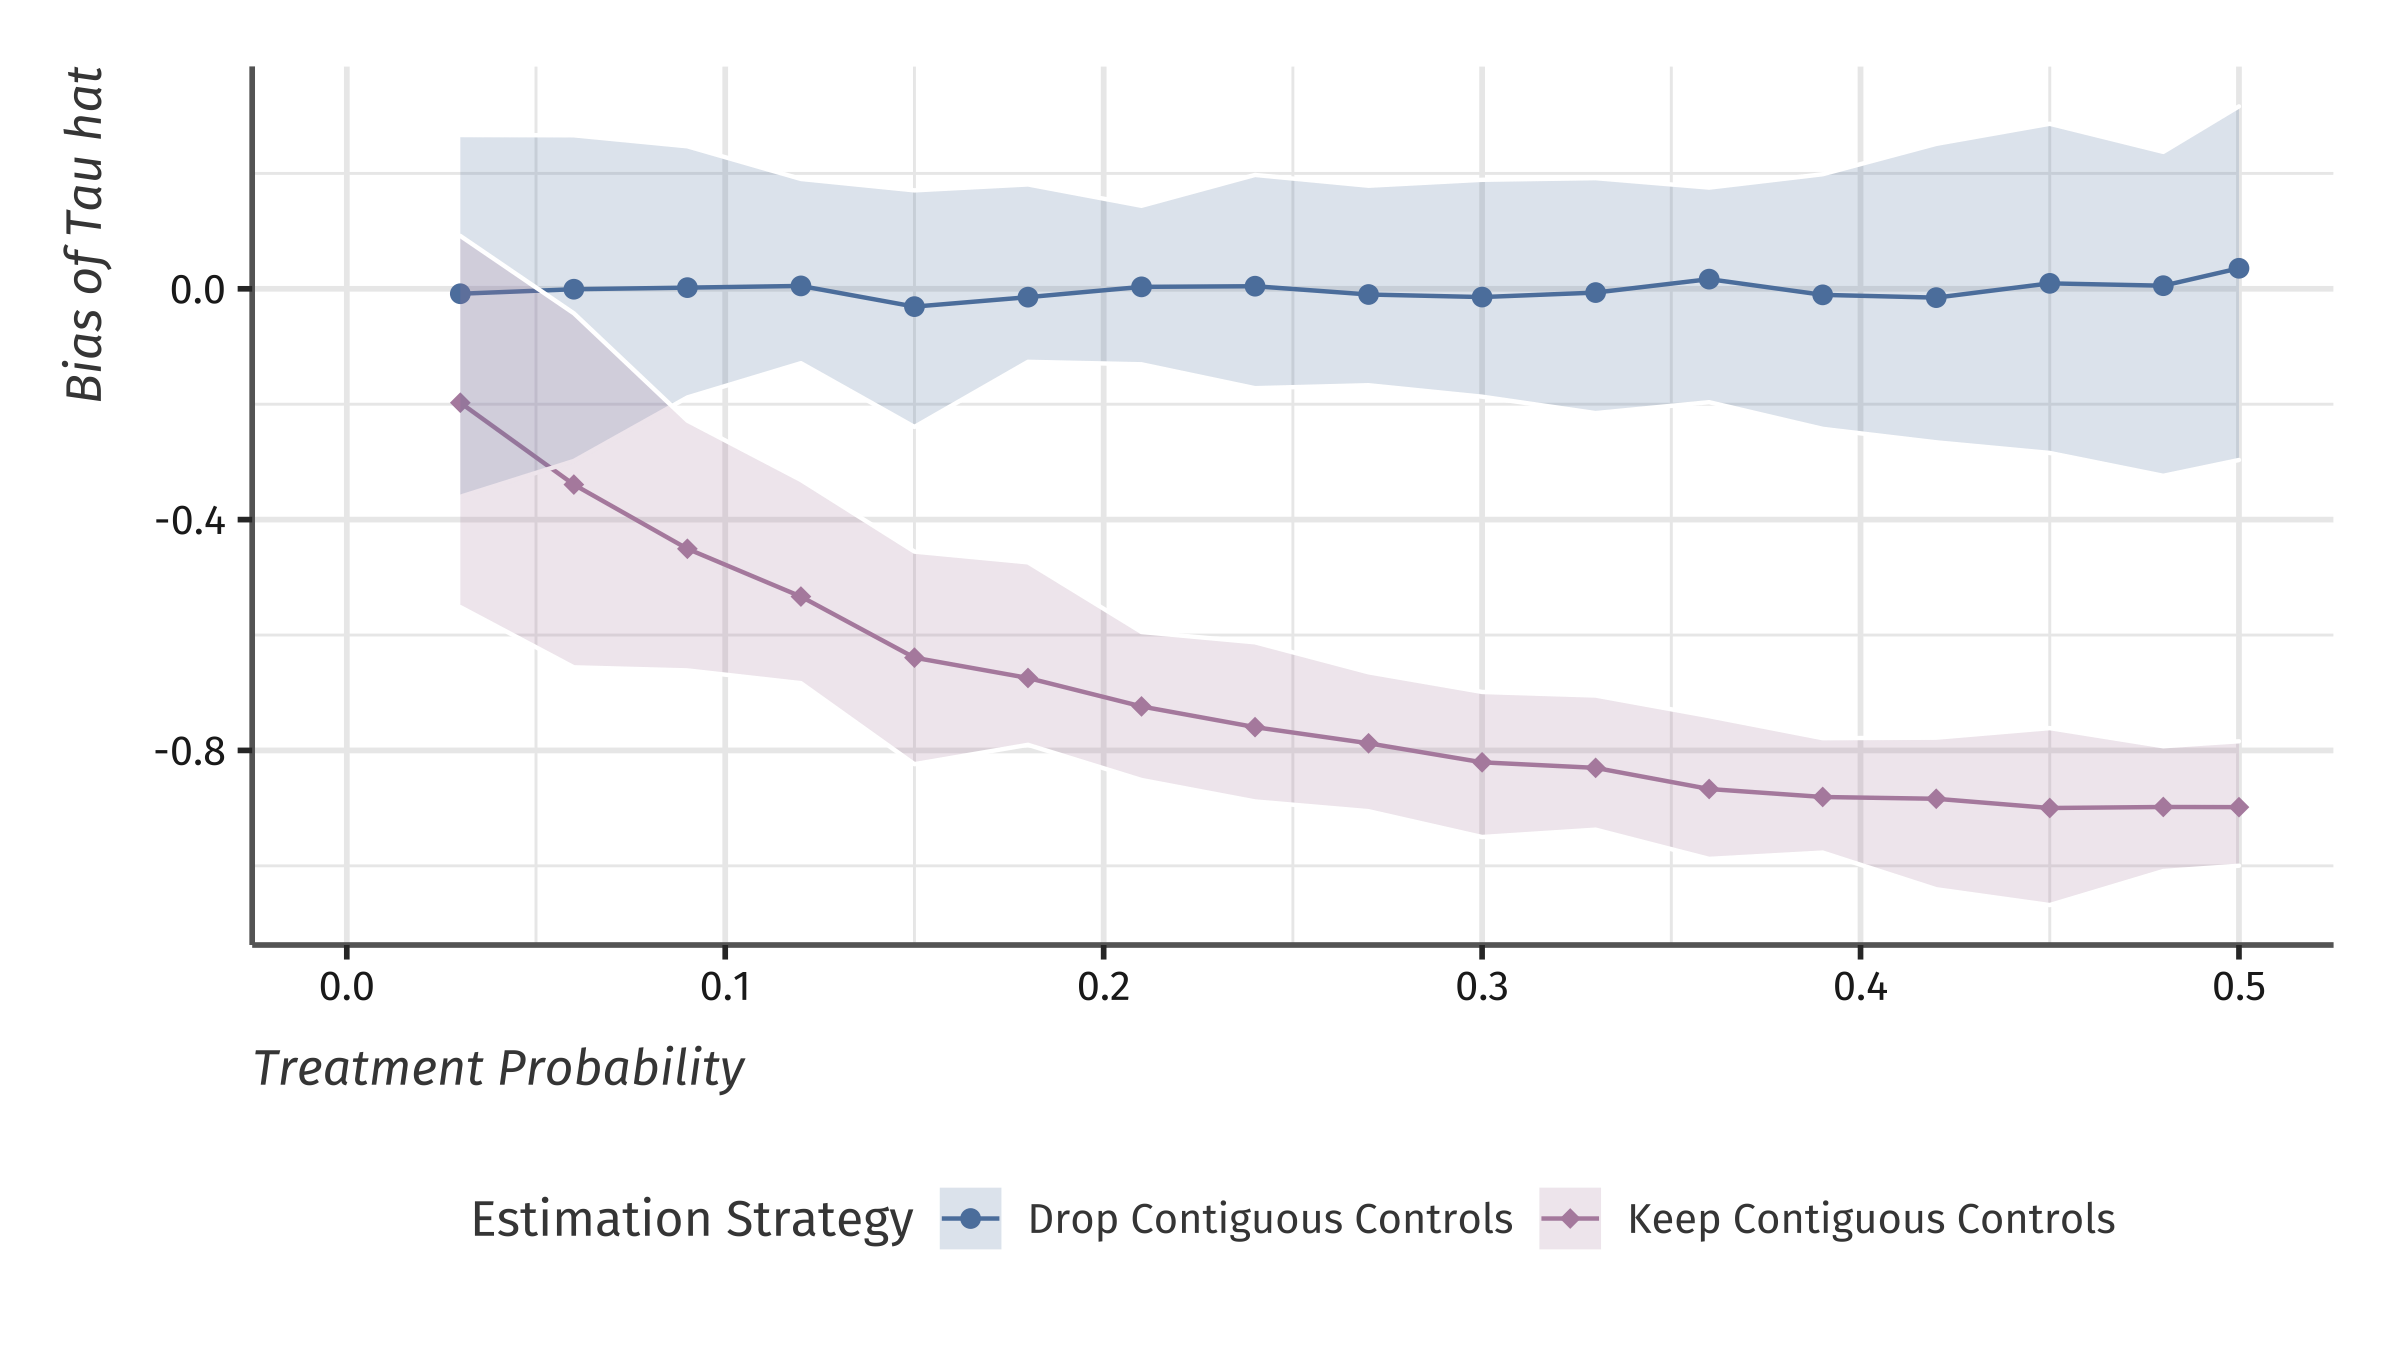
\includegraphics{../../figures/figure-bias_fix.png}
        } 
    }

    {\footnotesize
        \textit{Notes:} This figure plots the bias of $\hat{\tau}$ found from estimating Equation \ref{eq:twfe} for data generated as described in the text and Equation \ref{dgp1}. Each point corresponds to the average bias for the given treatment probability and the band is the 95 percent empirical confidence interval over 1000 simulations. The line with diamond markers estimates with all control units. The line with circle markers removes control units that share a border with a treated county. 
    }
\end{figure}

I now turn to a series of Monte Carlo Simulations to highlight the importance for controlling for spillovers in simulations. The data generating process used is defined by the exposure mapping given in Equation \ref{eq:example_exposure} and the data generating process given in Equation \ref{eq:example_po}. A unit of observation is a US county and the periods are $t \in \{1, \dots, 20\}$ with treatment turning on in period $t = 10$. The intercepet is $\alpha = -2$, the fixed effects are $\mu_t \sim N(t * 0.2, 0.1^2)$ and $\mu_i \sim N(6, 2^2)$, and the error term is $\epsilon \sim N(0, 2^2)$. Last, the size of treatment and spillovers are as follows: $\beta_{\text{direct}} = 2$, $\beta_{\text{spillover, control}} = 1$ and $\beta_{\text{spillover, treat}} = 0$.

For the first simulation, I restrict spillovers only to occur among control units, i.e. $\tau_{\text{spillover, treat}} = 0$ and estimate the typical two-way fixed effects model. This data generating process where spillovers only occur onto control units matches what has been typically assumed in the literature. I assign treatment among U.S. counties randomly with various probabilities between 3 percent and 50 percent. The DGP is therefore 
\begin{equation}
    \label{dgp1} 
    y_{it} = -2 + \mu_t + \mu_i + 2 D_{it} - (1-D_{it}) \text{Near}_{it} + \varepsilon_{it}   
\end{equation}

The size of the bias from estimating Equation \ref{eq:twfe} at different treatment probabilities are presented in Figure \ref{fig:bias_as_treat_prob} as the line with diamond markers. As displayed in the figure, even for a low treatment probability of three percent, the bias is quite large with a 95 percent empirical confidence interval between -0.28 and -0.75. As treatment frequency increases, the bias increases as well but at a slower rate due to fewer additional control units receiving spillover units. 

A common solution in the literature is to remove control units from the estimated sample that are most likely to be affected by spillovers. I do this in Figure \ref{fig:bias_as_treat_prob} and the results are shown by the line with circle markers. Even though, I remove contiguous controls which is not hte correct measure of $h_i(\vec{D}$, it approximates it well enough such that the bias stays centered constantly around zero as most control units experiencing spillovers are removed. As the portion of control units receiving spillovers that are kept in the sapmle increases, the bias would fall between the two lines.

There is a trade-off between the bias and the variance of the estimator when using this methodolgy. As the treatment probability increases, the number of control units removed increases as well. This naturally yields are more variable estimator as seen in the wider 95 percent empirical confidence intervals. 


% --------------------------------------------------
\subsection{Simulation 2}
% --------------------------------------------------

For the following simulation, I will add in spillovers onto also treated units with $\beta_{\text{spillover, treat}} = -0.5$. The DGP is as follows 
\begin{equation}
    \label{dgp2} 
    y_{it} = -2 + \mu_t + \mu_i + 2 D_{it} - (1-D_{it}) \text{Near}_{it} - 0.5 D_{it} \text{Near}_{it} + \varepsilon_{it}   
\end{equation} 
The proportion of treated units affected by the spillover depends on the spatial autocorrelation of the treatment assignment. In empirical applications, it is often the case that treatment assignment is concentrated in specific areas which yields higher proportion of treated units receiving spillover effects.

\begin{figure}[t]
    \caption{Example of Kriging Field}
    \label{fig:kriging}
    {\centering
        \resizebox{\columnwidth}{!}{
            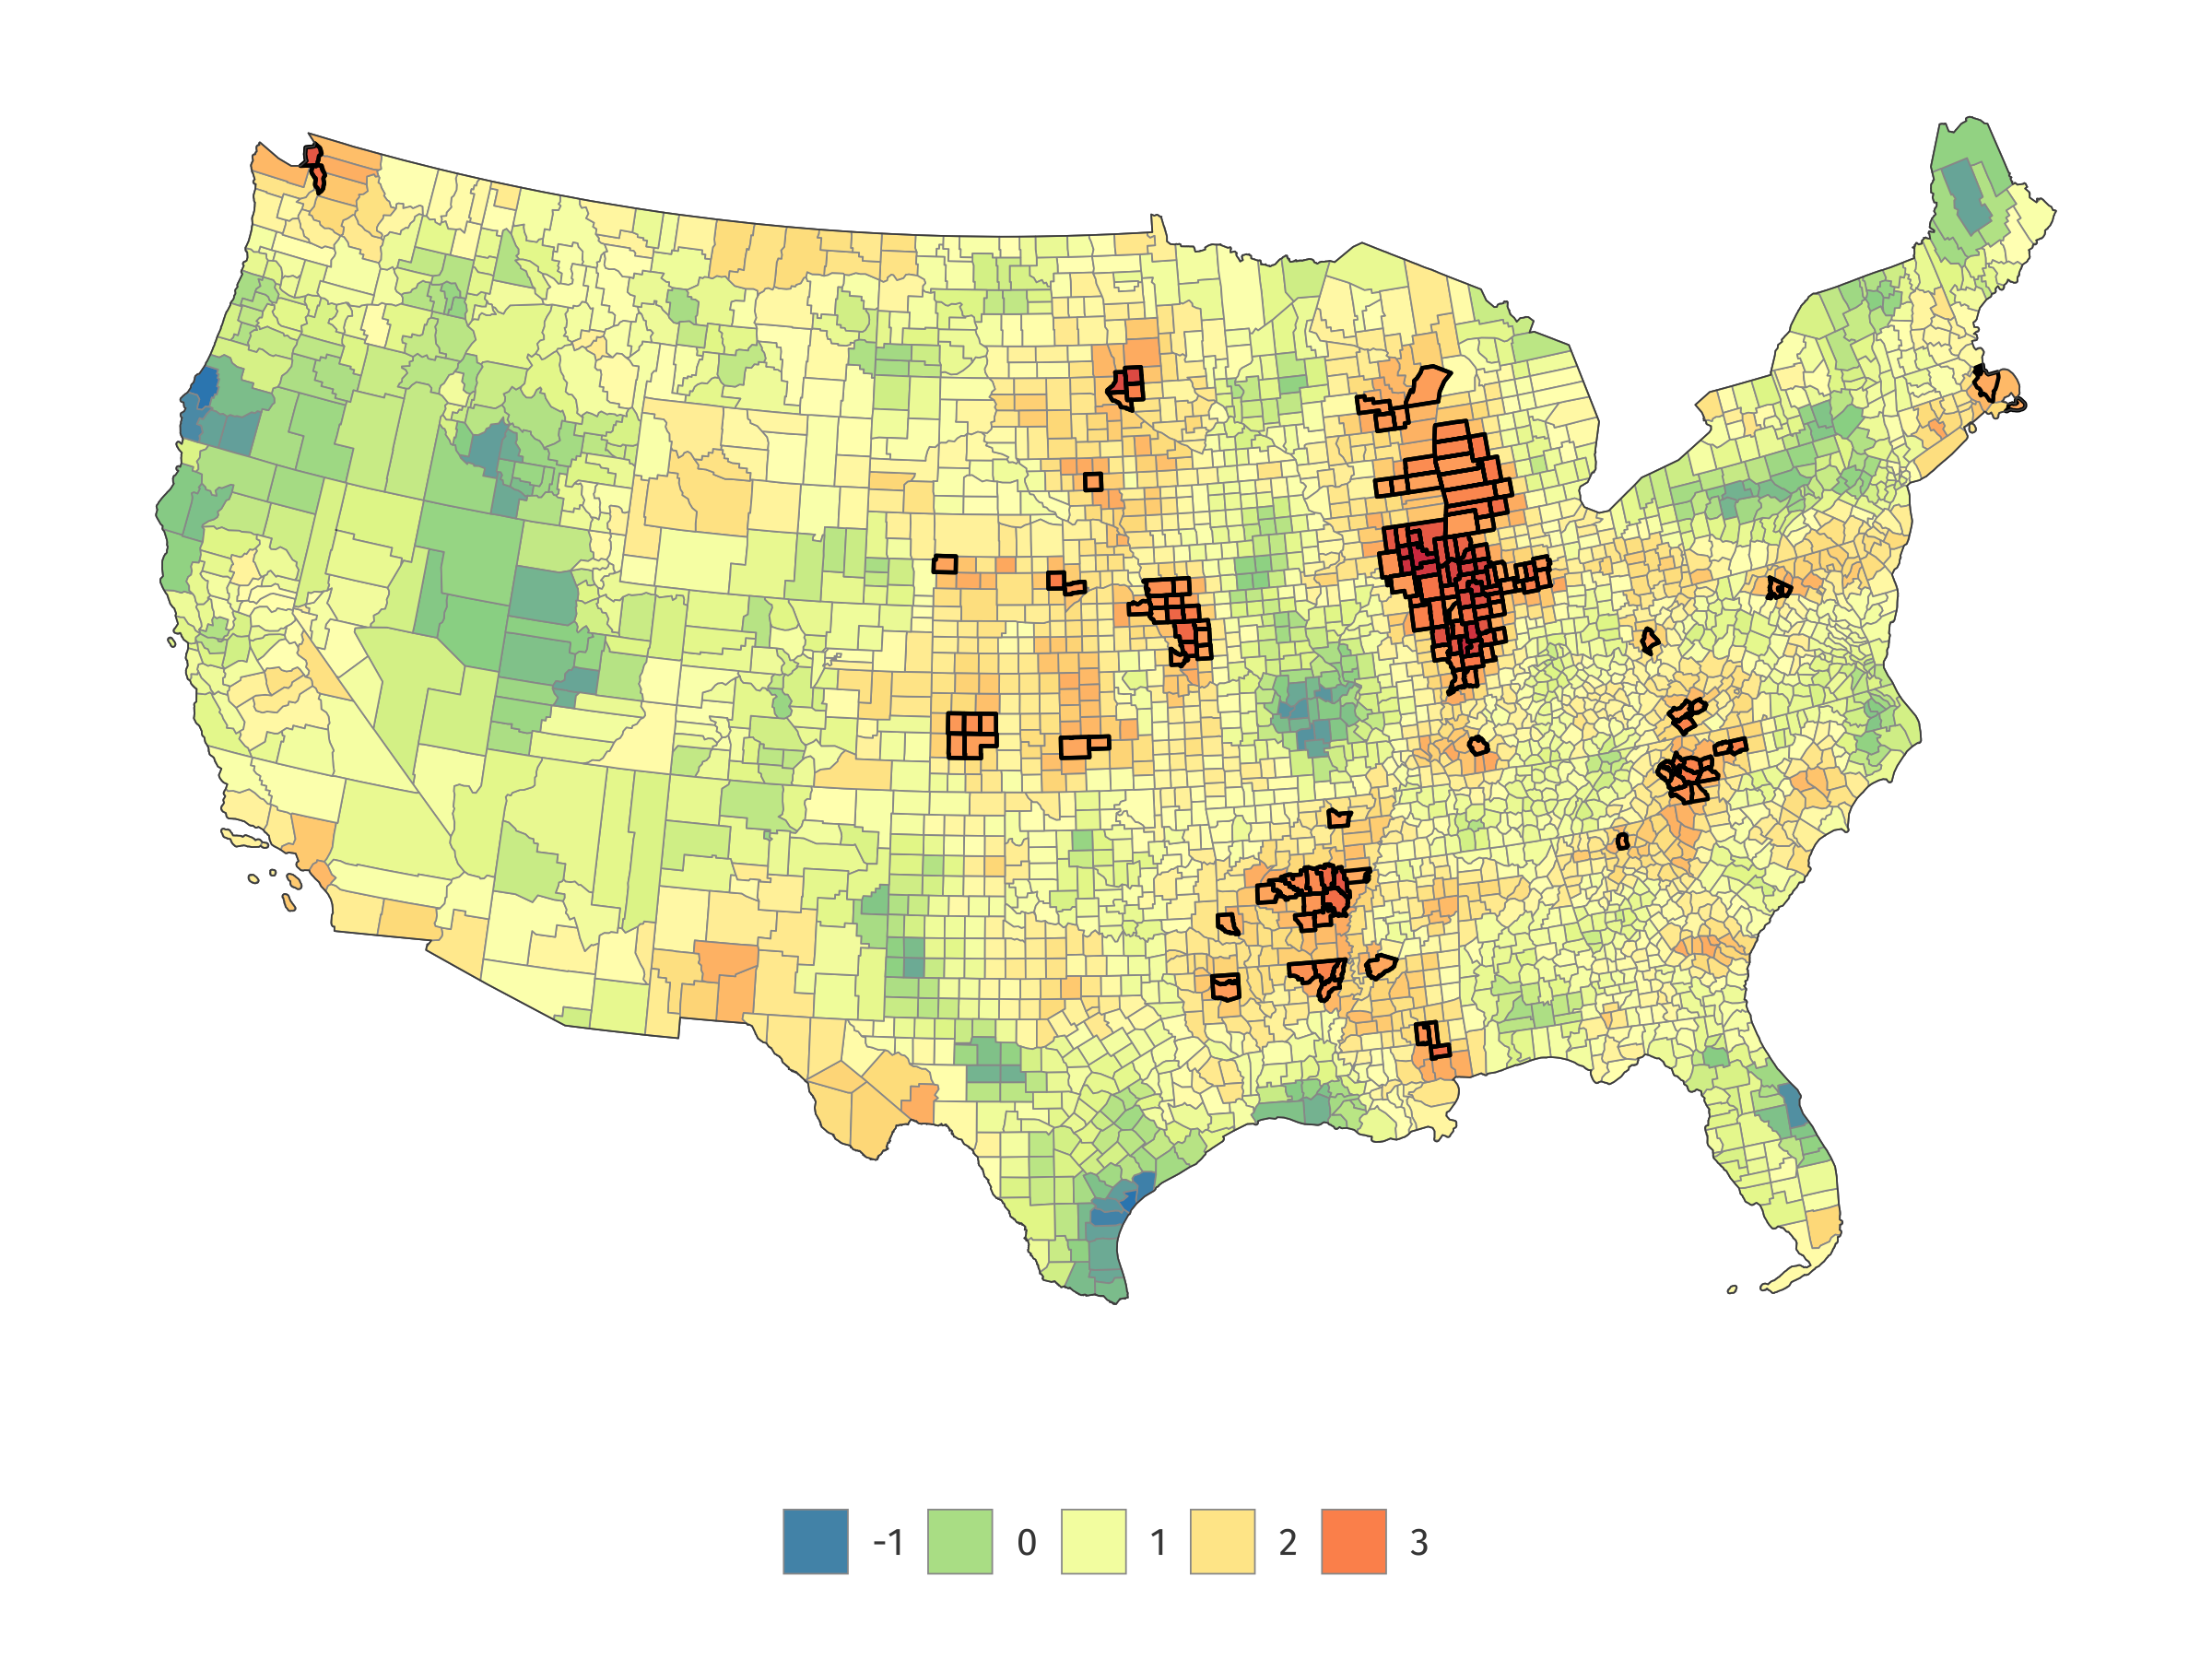
\includegraphics{../../figures/figure-krig.png}
        } 
    }
    {\footnotesize
        \textit{Notes:} This figure plots an example of a kriging simulation using the `gstat' package in R using an exponential variogram. The outlined counties are in the top ten percent of values for this simulation. 
    }
\end{figure}

In order to model spatial autocorrelation of treatment, I turn to a method from geosciences called `kriging'. Kriging generates a Gaussian field for a large grid of points across the entire United States where the spatial autocorrelation of the points is described by a set of parameters. One such field is depicted in Figure \ref{fig:kriging}. For a given field, I find the counties in the top ten percent of values and give these counties a value of $\text{Zone}_i = 1$. Then I assign treatment with a probability that differs based on Zone. The unconditional probability is equal to 5 percent in all simulations. To do this, I use a variable `Zone Plus' to adjust the relative probability of receiving treatment: 
\begin{equation}
    \label{eq:cond_prob}
    P(D_i \ \vert \ \text{Zone}_i) = (.1 + \text{Zone Plus} * \text{Zone}_i) \frac{.05}{.1 * .9 + (.1 + \text{Zone Plus}) * .1}
\end{equation}
The second term normalizes probabilities so the unconditional probability stays at 5 percent. In our simulations, Zone Plus ranges from 0 which is the case where p = 10 percent for all counties to 2 which has $P(D_i \ \vert \ \text{Zone}_i) = 0.166 + 0.35 * \text{Zone}_i$

\begin{figure}[t]
    \caption{Bias of $\hat{\tau}$ at Different Levels of Spatial Autocorrelation}
    \label{fig:bias_spatial_autocorr}
    {\centering
        \resizebox{\columnwidth}{!}{
            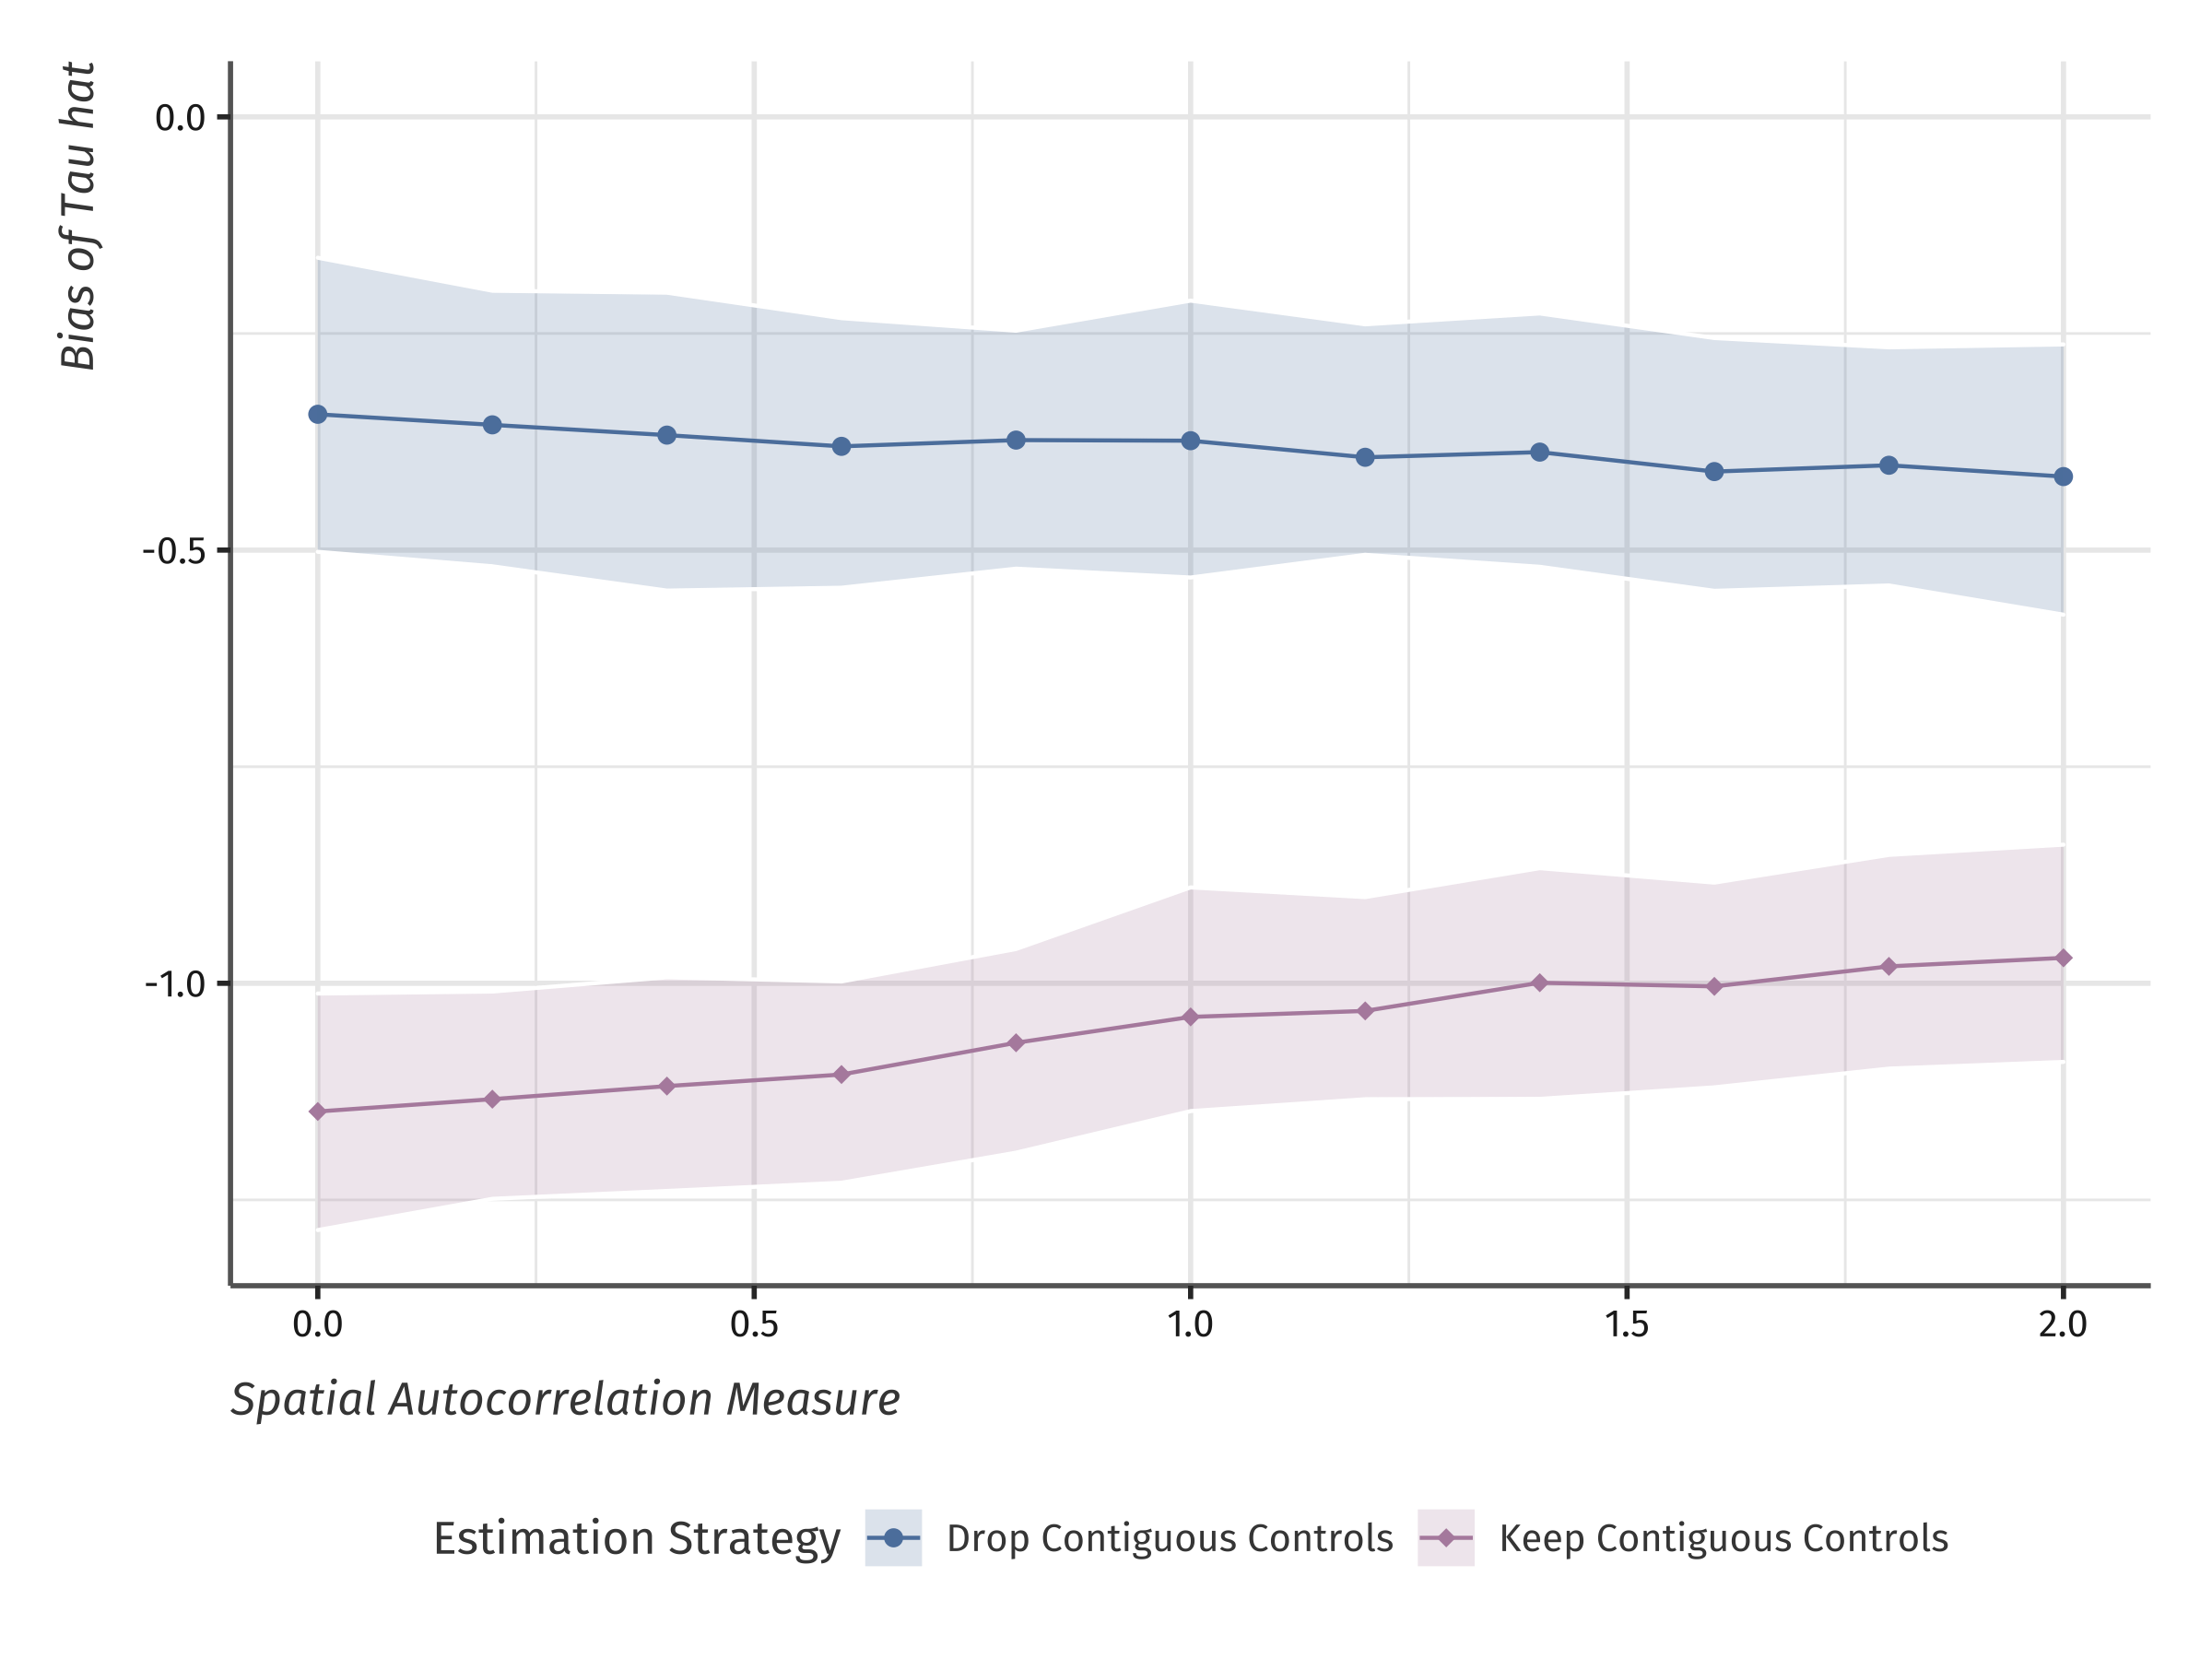
\includegraphics{../../figures/figure-bias_fix_spatial_autocorr.png}
        } 
    }
    {\footnotesize
        \textit{Notes:} This figure plots the bias of $\hat{\tau}$ found from estimating Equation \ref{eq:twfe} for data generated as described in the text and Equation \ref{dgp2}. Treatment probability is assigned according to the method described by the text and Equation \ref{eq:cond_prob}. Each point corresponds to the average bias for the given Zone Plus and the band is the 95 percent empirical confidence interval over 1000 simulations. The line with diamond markers estimates with all control units. The line with circle markers removes control units that share a border with a treated county. 
    }
\end{figure}

The results for the bias of $\hat{\tau}$ are in Figure \ref{fig:bias_spatial_autocorr}. The line with diamond markers is run on the full sample. As the level of spatial autocorrelation increases, the bias actually decreases. The reason for this is that as treatment becomes more concentrated in the `Zones', the number of control units receiving spillovers decreases while the number of treated units receiving spillovers increases. In this particular DGP, the effect of fewer control units on the bias is larger than the bias from more treated units. 

The line with circle markers in Figure \ref{fig:bias_spatial_autocorr} repeats the exercise of dropping control units that share a border with treated units. In the case where spillovers occur on treated units, all bias is not removed when dropping control units. That is because we only remove $\tau_{\text{spill,control}}$ but $\tau_{\text{spill,treated}}$ remains. To remove the second source of bias, it is necessary to acount directly for spillovers in the estimation strategy. I turn to this next. 






















% --------------------------------------------------
\newpage \printbibliography
% --------------------------------------------------


% --------------------------------------------------
\newpage \appendix 
\renewcommand{\thetable}{\Alph{section}.\arabic{table}}
% --------------------------------------------------

% --------------------------------------------------
\section{Proofs}
% --------------------------------------------------

\textbf{Proof of Theorem \ref{thm:bias}}
\begin{align*}
    \mathbb{E}_i\left[ \hat{\tau} \right] &= \mathbb{E}_i\left[ Y_{i1} - Y_{i0} \mid D_i = 1 \right] - \mathbb{E}_i\left[ Y_{i1} - Y_{i0} \mid D_i = 0 \right] \\
    &= 
    \mathbb{E}_i\left[ Y_{i1}(1, h_i(\vec{D})) - Y_{i0}(0, \vec{0})  \mid D_i = 1 \right] - \mathbb{E}_i\left[ Y_{i1}(0, h_i(\vec{D})) - Y_{i0}(0, \vec{0}) \mid D_i = 0 \right] \\
    &= 
    \mathbb{E}_i\left[ Y_{i1}(1, h_i(\vec{D})) - Y_{i0}(0, \vec{0})  \mid D_i = 1 \right] - \mathbb{E}_i\left[ Y_{i1}(0, h_i(\vec{D})) + Y_{i1}(0, \vec{0}) - Y_{i1}(0, \vec{0}) - Y_{i0}(0, \vec{0}) \mid D_i = 0 \right] \\
    &= 
    \mathbb{E}_i\left[ Y_{i1}(1, h_i(\vec{D})) - Y_{i0}(0, \vec{0})  \mid D_i = 1 \right] - \mathbb{E}_i \left[ Y_{i1}(0, \vec{0}) - Y_{i0}(0, \vec{0}) \mid D_i = 0 \right] \\ 
    &\quad - \mathbb{E}_i \left[ Y_{i1}(0, h_i(\vec{D})) - Y_{i1}(0, \vec{0})\mid D_i = 0 \right] \\ 
    &= 
    \mathbb{E}_i\left[ Y_{i1}(1, h_i(\vec{D})) - Y_{i0}(0, \vec{0})  \mid D_i = 1 \right] - \mathbb{E}_i \left[ Y_{i1}(0, \vec{0}) - Y_{i0}(0, \vec{0}) \mid D_i = 1 \right] \\
    &\quad - \mathbb{E}_i \left[ Y_{i1}(0, h_i(\vec{D})) - Y_{i1}(0, \vec{0})\mid D_i = 0 \right] \\  
    &= \mathbb{E}_i\left[ Y_{i1}(1, h_i(\vec{D})) - Y_{i0}(0, \vec{0}) - Y_{i1}(0, \vec{0}) + Y_{i0}(0, \vec{0})\mid D_i = 1 \right] - \mathbb{E}_i \left[ Y_{i1}(0, h_i(\vec{D})) - Y_{i1}(0, \vec{0})\mid D_i = 0 \right]\\
    &= \mathbb{E}_i\left[ Y_{i1}(1, h_i(\vec{D})) - Y_{i1}(0, \vec{0}) \mid D_i = 1 \right] - \mathbb{E}_i \left[ Y_{i1}(0, h_i(\vec{D})) - Y_{i1}(0, \vec{0})\mid D_i = 0 \right]\\
    &= \mathbb{E}_i\left[ Y_{i1}(1, h_i(\vec{D})) + Y_{i1}(1, \vec{0}) - Y_{i1}(1, \vec{0}) - Y_{i1}(0, \vec{0})\mid D_i = 1 \right] - \mathbb{E}_i \left[ Y_{i1}(0, h_i(\vec{D})) - Y_{i1}(0, \vec{0})\mid D_i = 0 \right]\\
    &= 
    \mathbb{E}_i \left[ Y_{i1}(1, \vec{0}) - Y_{i1}(0, \vec{0}) \mid D_i = 1 \right] + \mathbb{E}_i \left[ Y_{i1}(1, h_i(\vec{D})) - Y_{i1}(1, \vec{0}) \mid D_i = 1 \right] \\
    &\quad - \mathbb{E}_i \left[ Y_{i1}(0, h_i(\vec{D})) - Y_{i1}(0, \vec{0}) \mid D_i = 0 \right] \\
    &= \tau_{\text{direct}} + \tau_{\text{spill,treated}} - \tau_{\text{spill,control}}
\end{align*}








\end{document}